%% Slide 1.
\begin{frame}
\begin{itemize}[<+->]
\item
Beginning in 1997 with the publication of an NRC report titled \emph{``Modeling
and Simulation --- Linking Entertainment and Defense''}, the video game
community has pushed into spaces previously the domain of the VR community.
\item
Because much of the research
and development being conducted in the games community parallels the VR
community’s efforts, it has the potential to affect a greater audience.
\item
Researchers who want their work to remain relevant must realign to focus on
game research and development. Research in the games arena affects not just
the entertainment industry but also the government and corporate organizations
that could benefit from the training, simulation, and education opportunities
that serious games provide.
\end{itemize}
\end{frame}

\subsection{Defining Serious Games}

%% Slide 2.
\begin{frame}
\frametitle{What is a game?}
\begin{block}{A Dictionary Definition}
A physical or mental contest, played according to specific rules,
with the goal of amusing or rewarding the participants.
\end{block}
\pause
\begin{block}{A Video Game Definition}
A game played \alert{against a computer}, which would more
accurately be worded as a game played \alert{with a computer}.
\end{block}
\end{frame}

%% Slide 3
\begin{frame}
\frametitle{What is a serious game?}
\begin{block}{A Serious Game Definition}
A mental contest, played with a computer in accordance with
specific rules, \alert{that uses entertainment to} further government or
corporate training, education, health, public policy, and strategic
communication objectives.
\end{block}
\pause
\begin{block}{A Developer Definition}
Bing Gordon, chief creative officer of video and
computer games developer Electronic Arts, once
told that he defines video games as \alert{``story, art,
and software''}.
\end{block}
\end{frame}

%% Slide 4.
\begin{frame}
\frametitle{What is a serious game?}
\framesubtitle{Serious games have more than just story, art, and
software, however.}
\begin{center}
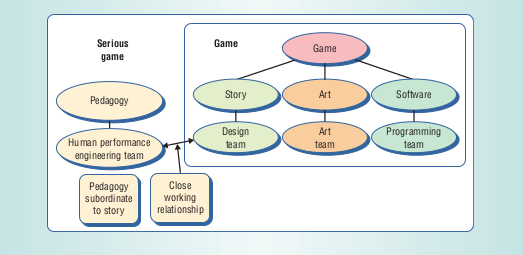
\includegraphics[scale=.75]{serious.png}
\end{center}
\end{frame}

\subsection{Creating a Science of Games}

%% Slide 5.
\begin{frame}
\frametitle{Creating a Science of Games}
\framesubtitle{Growing Interest}
\begin{itemize}[<+->]
\item
The development and wide release of the America's Army game began a
\alert{revolution} in thinking about the potential role of video games for
\alert{nonentertainment} domains.
\item
Those who have grown up playing games indicated that a game-centered research
and educational program could offer many positive benefits.
\item
The announcement of America's Army at the 2002 Electronics Entertainment Expo
(E3) prompted the US Army to commission a study of the game to see if it could
be used for training.
\end{itemize}
\end{frame}

%% Slide 6.
\begin{frame}
\frametitle{Creating a Science of Games}
\framesubtitle{An America's Army History}
\begin{itemize}
\item <1->
In the summer of 2002, a US Army captain from Fort Benning indicated that there
``was insufficient fidelity in the game for it to be of any use in training''.
\item <2->
In October 2002, when a staff sergeant from Fort Benning approached the
America's Army booth, an enthusiastic gamer who had played the game from
day one, he told the staff, ``We love this game at Benning. We use it for
training''.
\end{itemize}

\begin{block}{``Street finds its own use for things''}<3->
The sergeant had bypassed the Army's requirements documents and formal studies
and deployed the game on his own initiative.
\end{block}
\end{frame}


\subsection{Game Research Agenda}

%% Slide 7.
\begin{frame}
\frametitle{Game Research Agenda}
\framesubtitle{}
\begin{block}{
To influence the future of both serious and entertainment games}
Developers must create a research and development agenda with three components:
\begin{itemize}
\item <2->
infrastructure;
\item <3->
cognitive game design;
\item <4->
immersion.
\end{itemize}
\end{block}
\end{frame}

%% Slide 8.
\begin{frame}
\frametitle{Game Research Agenda}
\framesubtitle{Infrastructure}
The underlying software and hardware necessary for developing interactive
games include \alert{MMOG architectures}, game engines and tools,
streaming media, next-generation consoles, wireless and mobile device.
\pause
\begin{block}{}
MMOGs pose the fundamental research
question of how to develop dynamically extensible
and semantically interoperable software architectures.
\end{block}
\pause
\vfill
This work, of interest to gaming in general, has special relevance for the
large governmental game-based simulation sector.
\end{frame}

%% Slide 9.
\begin{frame}
\frametitle{Game Research Agenda}
\framesubtitle{Cognitive Game Design and Immersion}
\begin{block}{Cognitive Game Design:}
\begin{itemize}
\item
modeling and simulating computer characters,
story, and human emotion;
\item
analyzing large-scale game play;
\item
innovating new game genres and play styles;
\item
integrating pedagogy with story in the interactive game medium.
\end{itemize}
\end{block}

\pause

\begin{block}{Immersion:}
\begin{itemize}
\item
computer graphics, sound, and haptics;
\item
affective computing—sensing human state and
emotion;
\item
advanced user interfaces.
\end{itemize}
\end{block}
\end{frame}
